\section{Storing, representing, and converting multimedia data}
\label{sec:storing}

As you may have imagined, a book about computational analysis of \textit{communication} would be incomplete without a chapter dedicated to conduct analysis over other unstructured data formats different from text. In fact, if you think of the possible contents derived from social, cultural and political dynamics in the current digital landscape, you will realize that written contents are only a limited (though potential) slide of the bigger cake. Humans produce much more oral contents than text messages, and are more agile in deciphering sounds and visual contents. Digitalization of social and political life, as well as the explosion of self-generated digital contents in the web and social media, have provoked an unprecedented amount of multimedia contents that deserve to be include in many types of research.

Just imagine a collection of digital recorded radio stations, or the enormous amount of pictures produced everyday in Instagram, or even the millions of videos of social interest uploaded in Youtube. These are definitely goldmines for social researchers who traditionally used manual techniques to analyse just a very small portion of these multimedia contents. However, it is also true that computational techniques to analyze audio, images or video are still little developed in social sciences given the the difficulty of application for non-computational practitioners and the novelty of the discoveries in fields such as computer vision. 

This section gives a brief overview over different formats of multimedia files, in special images, vector graphics, bitmaps, and related concepts. We explain how to generate useful inputs into our pipeline to perform computational analysis.

You are already probably familiar with digital formats of images (.jpg, .bmp, .gif, etc.), audio (.mp3, .wav, .wma, flac, etc.) or video (.avi, .mov, .wmv, .flv, etc.), which is the very first step to use these contents as input. However, similarly to the case of texts you will need to do some preprocessing to put these formats into shape and get a proper mathematical representation of the contents. 

In the case of audio, there might be many useful computational approaches to do research over these contents: from voice recognition, audio sentiment analysis or sound classification, to automatic generation of music. Recent advances in the field of artificial intelligence have created a prosperous and diversified field with multiple academic and commercial applications. Nevertheless, computational social scientists can obtain great insights just by using specific applications such as speech-to-text transformation and then apply text analytics (already explained in this book) to the results. As you will see in the next section (\refsec{ocr}), there are some useful libraries in R and Python to use pre-trained models to transcribe voice in different languages. Even when this approach is quite limited (just a small portion of the audio analytics world) and constrained (we will not address how to create the models), it will show how a specific, simple and powerful application of the automatic analysis of audio inputs can help answering many social questions (i.e. what are the topics of a natural conversation, what are the sentiments expressed in the scripts of radio news pieces, or which actors are named in oral speeches of any political party).

On the other hand, applying computational methods to video inputs is probably the most challenging task in spite of the recent and promising advances in computer vision. For the shake of space, we will not cover specific video analytics in this chapter, but it is important to let you know that most of the computational analysis of video is based on the inspection of image and audio contents. With this standard approach you need to specify which key frames you are going to extract from the video (for example take an still image every 1,000 frames) and then apply computer vision techniques (such as object detection) to those independent images. Check for example the the version 3 of the object detection architecture \textit{You Only Look Once Take} (YOLOv3)\footnote{https://pjreddie.com/darknet/yolo/} created by \citet{yolov3}, which uses a pre-trained Convolutional Neural Network (CNN) (see section \refsec{cnn}) to locate objects within the video (figure~\ref{fig:yolo}). To answer many social science questions you might complement this frame-to-frame image analysis with a basic analysis of audio features derived from a speech-to-text task. In any case, this approach will not cover some interesting aspects of the video such as the camera frame shots and movements, or the editing techniques, which certainly give more content information.

\begin{figure}
\centering
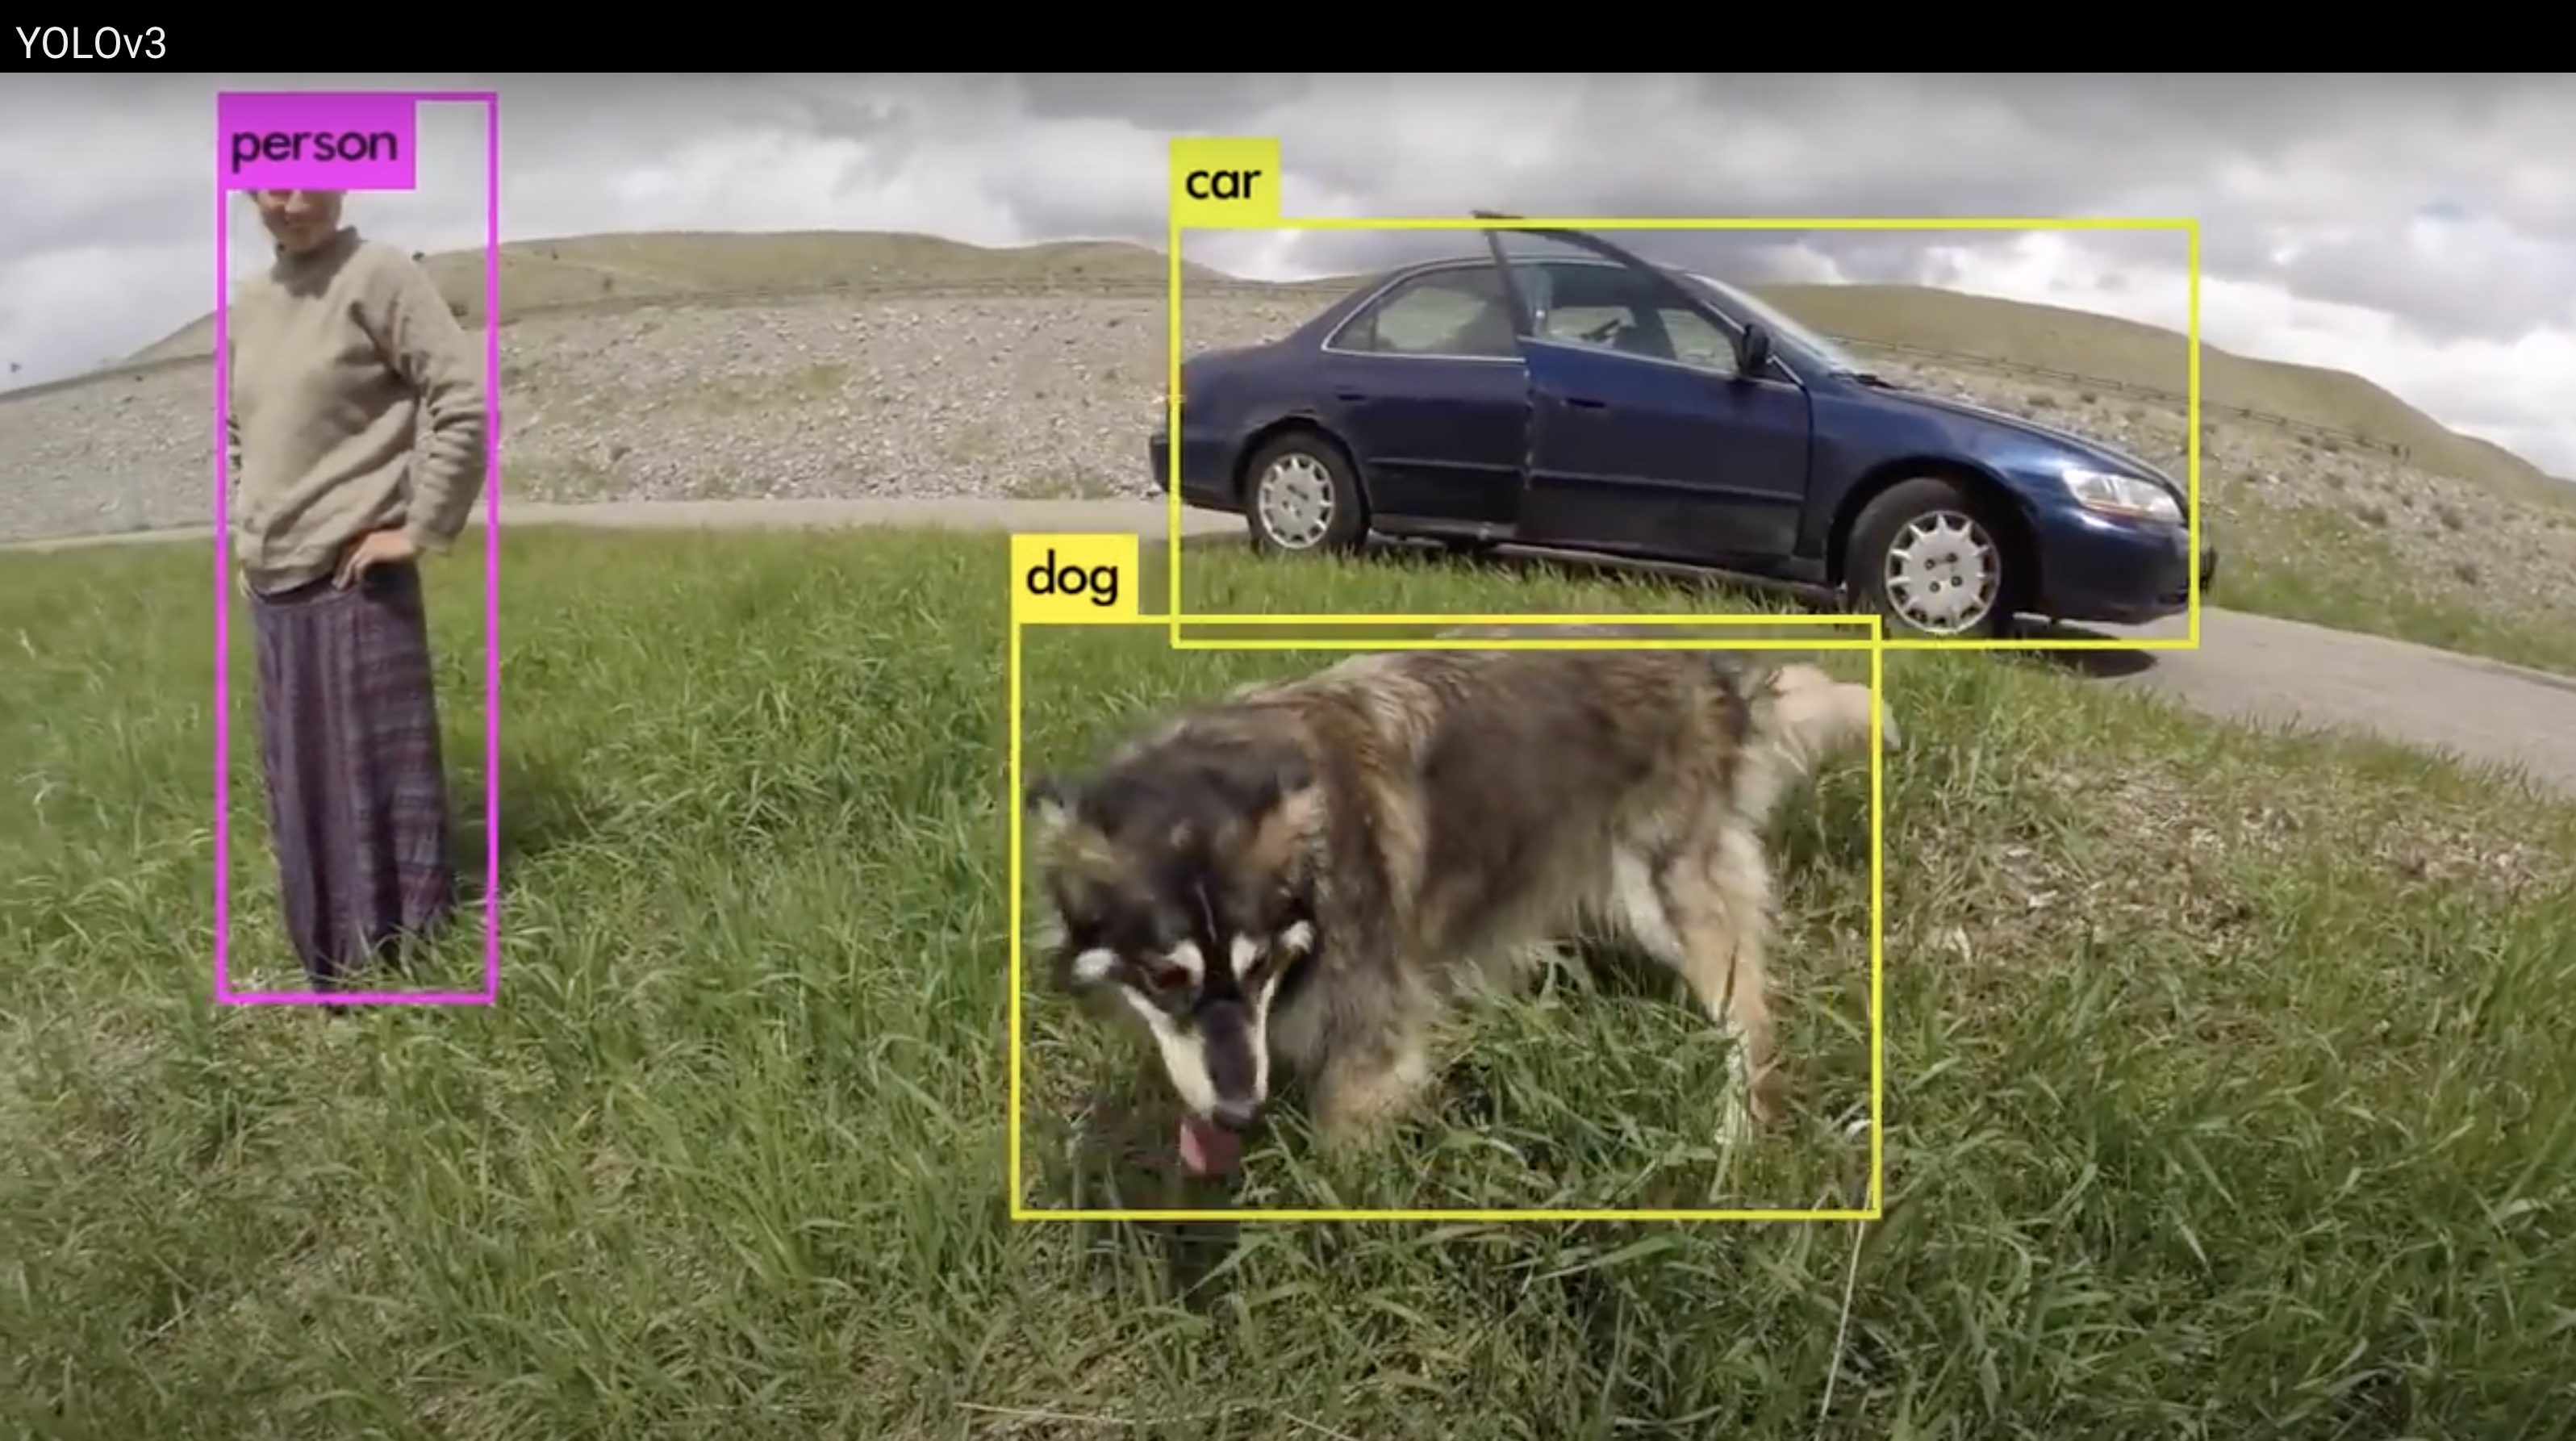
\includegraphics[width=0.9\linewidth]{figures/ch15_yolo.png}
\caption{A screen shot of a real-time video analyzed by YOLOv3 in its webpage https://pjreddie.com/darknet/yolo/}
\label{fig:yolo}
\end{figure}

Thus, we will focus in this section in learning how to store, represent, and convert images for further computational analysis. You can also have a very nice and complete overview of computational analysis of images in WEBB, CASAS & WILKERSON (forthcoming XXX).

To perform basic image manipulation we have to: (i) load images and transform their shape when it is necessary (by cropping or resizing), and (ii) to create a mathematical representation of the image (normally derived from it size, colors and pixel intensity) such of a 3D matrix or a flatten vector. You have some useful libraries in Python and R (\pkg{pil} and \pkg{imagemagik}, respectively) to conduct research in these initial stages, but you will also find that more advanced libraries in computer vision will include functions or modules for pre-processing images. At this point you can work either locally or remotely, but keep in mind that images can be heavy files and if you are working with thousands of files you will probably need to store or process them in the cloud (see Section~\ref{sec:cloudcomputing}).

You can load any image as an object onto your workspace as we show in \refex{load}. In this case we load and visualize two pictures of refugees published by mainstream media in Europe (see \citet{amores2019visual}), one is a JPG and the other is a PNG file. For this basic loading step we used the \fn{open} function of the \fn{Image} module in \pkg{pil} and \fn{image_read} function in \pkg{imagemagik}. The JPG image file is a 805x453 picture with the color model \textit{RGB} and the PNG is a 1540x978 picture with the color model \textit{RGBA}. As you may notice the two objects have different formats, sizes and color models, which means that there is little analysis you can do if you don't create a standard mathematical representation of both. 

\pyrex[output=both,caption=Loading JPG and PNG pictures as objects]{chapter15/load}

The good news when working with digital images is that the concept of \texttt{pixel} (picture element) will help you to understand the basic mathematical representation behind computational analysis of images. A rectangular grid of pixels is represented by a dot matrix which in turn generates a \texttt{bitmap image} or \texttt{raster graphic}. The dot matrix data structure is a basic but powerful representation of the images since we can conduct multiple simple and advanced operations with the matrices. Specifically, each dot in the matrix is a number that contains information about the intensity of each pixel (that commonly ranges from 0 to 255) also known as bit or color depth. This means that the numerical representation of a pixel can have 256 different values being 0 the darkest tone of a given color and 255 the lightest. Keep in mind that if you divide the pixel values by 255 you will have a 0-1 scale to represent the intensity.

In a blank-and-white picture we will only have one color (grayscale), with the darker points representing the black and the lighter ones the white. The mathematical representation will be a single matrix or a two-dimensional array in which the number of rows and columns will correspond to the dimensions of the image. For instance in a 224 x 224 black-and-white picture we will have 50,176 integers (0-255 scales) representing each pixel intensity. 

In \refex{imagel} we convert our original JPG picture to grayscale and then create an object with the mathematical representation (a 453 x 805 matrix).

\pyrex[output=both,caption=Converting images to grayscale and creating a two-dimensional array]{chapter15/imagel}

By contrast, colour images will have multiple color channels that depend on the color model you chose. One standard color model is the  three-channel RGB (\textit{red}, \textit{green} and \textit{blue}), but you can find other variations in the chosen colors and the number of channels such as: RYB (\textit{red}, \textit{yellow} and \textit{blue}), RGBA (\textit{red}, \textit{green}, \textit{blue} and \textit{alpha}\footnote{Alpha refers to the opacity of each pixel} ) or CMYK (\textit{cyan}, \textit{magneta}, \textit{yellow} and \textit{key}\footnote{Key refers to \textit{black}}).  For the case of RGB, the mathematical representation will be a three-dimensional matrix or a collection of three two-dimensional arrays (one for each color). Then a RGB 224 x 224 picture will have 50,176 pixel intensities for each of the three colors, or in other words a total of 150,528 integers!

Now, in \refex{imagergb} we convert our original JPG file to a RGB object and then create a new object with the mathematical representation (a 453 x 805 x 3 matrix).

\pyrex[output=both,caption=Converting images to RGB color model and creating three two-dimensional arrays]{chapter15/imagergb}

Instead of pixels, there are other ways to store digital images. One of them is the \textit{vector graphics}, with formats such as .ai, .eps, .svg or .drw. Differently to bitmap images, they don't have a grid of dots but a set of \textit{paths} (lines, triangles, square, curvy shapes, etc.) that have a start and end point, so simple and complex images are created with with paths. The great advantage of this format is that images do not get "pixeled" when you enlarge them because the paths can easily be transformed 	while remaining smooth. However, to obtain the standard mathematical representation of images you can easily convert (back and forth) the vector graphics to raster graphics such as RGB.

  
crop
resize
compare with Flatten vector
